%========= Introduction
\section{Introduction}
\label{sec:introduction}
One more paragraph?

\subsection{Aim \& Objectives}~\label{subsec:aims}
How about this paragraph in section 1.1!
\begin{figure}[h]
    \centering
    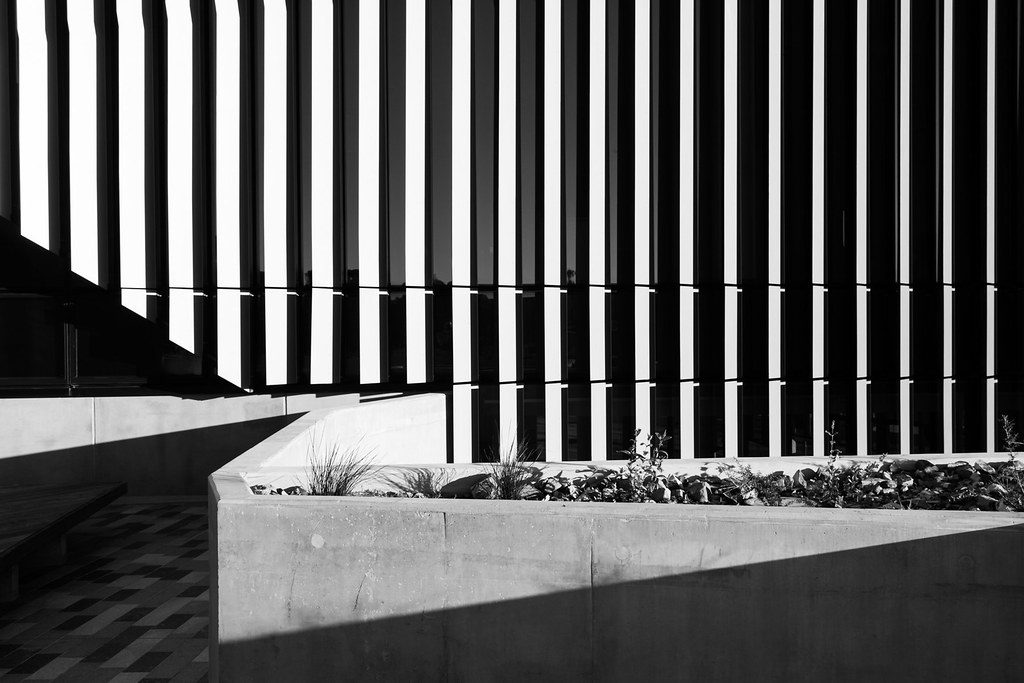
\includegraphics[width=0.7\textwidth]{Deakin_img.jpg}
    \caption{Deakin Campus Building.}
    \label{fig:building}
\end{figure}

Figure~\ref{fig:building} shows the Deakin BC building at Burwood campus in Melbourne.

\subsection{Structure}\label{subsec:structure}
Section~\ref{sec:literature} reviews the literature. Section~\ref{sec:design} presents the research design and methodology. Section~\ref{sec:approach} describes the approach and the technical details of artefact development. Section~\ref{sec:evaluation} evaluates the artefacts, on the basis of research questions (RQs) in Section~\ref{subsec:RQs} and discusses the RQs in Section~\ref{sec:discussion}. Section~\ref{sec:threats} discusses threats to validity and Section~\ref{sec:conclusion} concludes the report. 

\almarginpar{This paragraph can be removed}Here is how we cite a single reference captured in your file "zotero\_reference.bib" \cite{gameiro_research_2018}. We can cite multiple authors as well \cite{skolnik_radar_2008,the_joint_board_on_scientific_information_policy_radar_1945}. And if you want to cite something from a book which is large, or from a specific page of the paper, e.g. when we quote its part, then we'd better refer to  a section or a page numbers, e.g. "New radar technologies and applications are discovered and proposed almost every day; however, there still exists challenges and gaps that need to be addressed." \cite[p4]{stimson_introduction_1998}\todo{For other options check the \textbackslash cite macro for bibtex}.\todo{Is this the correct citation style? does it have to be Deakin Harvard: e.g., my reference (Author, 20XX)}
